\documentclass{article}
\usepackage{amsmath}
\usepackage{amsfonts}
\usepackage{tikz}

\usepackage[shortlabels]{enumitem}

\usepackage{algorithm}
\usepackage{booktabs}
\usepackage{algpseudocode}

\textwidth=7.6in
\textheight=9.9in
\topmargin=-.9in
\headheight=0in
\headsep=.5in
\hoffset=-1.5in
\setlength\parindent{0pt}


\begin{document}

\begin{center}
    \Large{\textbf{Problem Set 6 Solutions}} \\[0.25ex]
    Calvin Walker
\end{center}
\textbf{Problem 1}:

\begin{center}

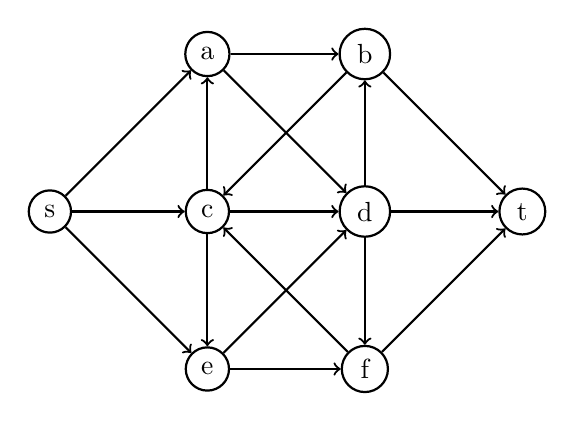
\begin{tikzpicture}[auto, node distance=2cm, every loop/.style={},
    thick,main node/.style={circle,draw},]

\node[main node] (s) {s};
\node[main node] (c) [right of=s] {c};
\node[main node] (a) [above of=c] {a};
\node[main node] (b) [right of=a] {b};
\node[main node] (d) [below of=b] {d};
\node[main node] (e) [below of=c] {e};
\node[main node] (f) [right of=e] {f};
\node[main node] (t) [right of=d] {t};

\path[every node/.style={font=\sffamily\small}]
(s) edge [->] node {} (a)
(s) edge [->] node {} (c)
(s) edge [->] node {} (e)

(a) edge [->] node {} (b)
(a) edge [->] node {} (d)

(b) edge [->] node {} (c)
(b) edge [->] node {} (t)

(c) edge [->] node {} (a)
(c) edge [->] node {} (e)
(c) edge [->] node {} (d)


(d) edge [->] node {} (f)
(d) edge [->] node {} (t)
(d) edge [->] node {} (b)

(f) edge [->] node {} (t)
(f) edge [->] node {} (c)

(e) edge [->] node {} (f)
(e) edge [->] node {} (d);

\end{tikzpicture}
\end{center}
\textbf{Problem 2}: \\[1.0ex]
\underbar{Algorithm}: If $e$ was not at full capacity, such that $f(e) < c_e$, then reducing $c_e$ by 1 will have no effect, so $F$ is unchanged. If $e$ is at full capacityy, there must be a path from $u$ to $s$ and a path from $t$ to $v$ in the residual graph. Traverse a path in the residual graph $t \rightarrow \dots \rightarrow v$ and a path $u \rightarrow \dots \rightarrow s$, and for each reverse edge, undo one unit of flow by decrementing the reverse edges and incrementing the forward edges. Do the same for $e$ unless the new capacity is zero, in which case both the forward and reverse edge $e^{\leftarrow}$ have capacity zero. Then, use one iteration of Ford-Fulkerson to find the new max-flow in the updated graph. \\[0.5ex]
\underline{Correctness}: Consider the algorithm in each of the possible scenarios
\begin{enumerate}
    \item $e$ was not at full capacity, so $f(e) < c_e$ and $f(e) \leq c_e - 1$, therefore the max-flow is unchanged.
    \item $e$ was at full capacity, and there is a path from $u$ to $v$ in the residual graph, so if capacity $c_e$ is decremented by one, we can route this unit of flow along the alternate path from $u$ to $v$ using Ford-Fulkerson, and the max-flow will be unchanged.
    \item $e$ was at full capacity, and there is not a path from $u$ to $v$ in the residual graph. 
    
    Since the flow into $u$ must equal the flow out of $u$, and $e$ has capacity at least $1$, there must be at least one path from $s$ to $u$ having positive flow. Thus, there is a path in the residual graph using reverse edges from $u$ to $s$. Similarly, the flow into $v$ must equal the flow out of $v$, and the same can be said for all verticies on a path from $v$ to $t$, so there must be a path from $v$ to $t$ having positive flow. Thus, there is a path in the residual graph using reverse edges from $t$ to $v$. 
    
    If we undo one unit of flow along each of these paths and undo one unit of flow through $e$, then we have a valid flow for the updated graph, since we have reduced the flow into and out of $e$ by one to satisfy its new capacity, and the Ford-Fulkerson algorithm can now find the updated max-flow.
\end{enumerate}
\underline{Runtime}: Since each edge in the updated graph had at most one unit of flow undone, the Ford-Fulkerson algorithm can find the new max-flow in one iteration, or $O(|E|)$, as it is at most one unit less than the original graph. We can traverse the residual graph to find and update the paths from $t$ to $v$ and from $u$ to $s$ in $O(|V| + |E|)$ time. So the total runtime is $O(|V| + |E|)$. \textit{change to 2 iterations?} \\[1.0ex]
\textbf{Problem 3}: \\[0.75ex]
\underbar{Algorithm}: Initialize a directed graph $G = (V, E)$ such that there is a vertex $s$ with edges to all $i \in [m]$ of capacity $s_i$, each vertex $i \in [m]$ has edges to all $j \in [n]$ with capacity $c_{ij}$, and all $j \in [n]$ have edges to a vertex $t$ with capacity $b_j$. Then, compute the max-flow from $s$ to $t$ using Ford-Fulkerson, and return the integer value of the flow as $T$. \\[0.5ex]
\underline{Proof}: Since the correctness of Ford-Fulkerson is accepted, we will prove the correctess of the algorithm by proving that this problem is reducible to max flow. Consider a sales plan $S$ with total sales $T = \sum_{i = 1}^{m}\sum_{j = 1}^{n}x_{ij}$. Let $(u, v)$ denote the edge between to verticies in $G$, where $c_{(u, v)}$ is the capactiy of $(u, v)$. If $S$ is a valid sales plan, then: 
\begin{itemize}
    \item For all $i \in [m]$, $\sum_{j}^{n} x_{ij} \leq s_i = c_{(s, i)}$, so the flow $f((s, i)) \leq c_{(s, i)}$
    \item For all $i \in [m]$ and $j \in [n]$, $ x_{ij} \leq c_{ij} = c_{(i, j)}$, so the flow $f((i, j)) \leq c_{(i, j)}$
    \item For all $j \in [n]$, $\sum_{i}^{m} x_{ij} \leq b_j = c_{(j, t)}$, so the flow $f((j, t)) \leq c_{(j, t)}$
\end{itemize}
So for every edge in $G$, no capacity is exceeded for sales plan $S$, so the flow where $f((i, j)) = x_{ij}$ has value $T$ in $G$. Now, assume there is an integer-valued flow with value $T$ in $G$. Then we take the sales plan $S = \{x_{ij} = f((i, j))\}$, which has total sales $T$. So there is a bijection between integer valued flows on $G$ and sales plans. Thus, the problem is reducible to max flow.\\[0.5ex]
\underline{Runtime}: We can initialize the graph $G$ in linear time. The maximum flow on $G$ is bound by the supply $S = \sum_{i}^{m}s_i$ and there are $mn + m + n$ edges in $G$. So Ford-Fulkerson will run in $O(Smn)$ time, giving the algorithim a runtime of $O(Smn)$. \\[1.0ex]
\textbf{Problem 4}:
\end{document}